\documentclass{beamer}
\mode<presentation> {
	\usetheme{Malmoe}
	\usecolortheme{whale}
	\setbeamertemplate{footline}[page number]
	\setbeamertemplate{navigation symbols}{}
}

\usepackage{graphicx} 	% Allows including images
\usepackage{booktabs} 	% Allows the use of \toprule, \midrule and \bottomrule in tables
\usepackage{tikz} 		% Pretty diagrams.
\usepackage{adjustbox}	% Scale images/diagrams to slide
\usepackage{color}
\usepackage{listings}
\usetikzlibrary{
	positioning				% Allows 5px above/below of x style positioning
	, arrows				% Allows <-, ->, <-> style arrows.
	, fit					% Allows fitting lines to shapes
	, decorations.pathreplacing	% Allows decoration that affect line paths.
	, backgrounds
	, shapes
	, shapes.multipart
	, calc
	, chains
}

\definecolor{dblue}{rgb}{0,0,0.545}
\definecolor{lgrey}{rgb}{0.9,0.9,0.9}
\definecolor{darkblue}{rgb}{0.0,0.0,0.6}
\lstdefinelanguage{nuclear}{
	backgroundcolor=\color{gray!10},  
	basicstyle=\footnotesize \ttfamily \color{black} \bfseries,   
	breakatwhitespace=false,	   
	breaklines=true,			   
	captionpos=b,				   
	commentstyle=\color{green!50!black},   
	deletekeywords={...},		  
	escapeinside={\%*}{*)},				  
	frame=single,				  
	language=C++,				
	keywordstyle=\color{violet},  
	morekeywords={constexpr}, 
	identifierstyle=\color{black},
	stringstyle=\color{red},	  
	numbers=left,				 
	numbersep=5pt,				  
	numberstyle=\tiny\color{black}, 
	rulecolor=\color{black},		
	showspaces=false,			   
	showstringspaces=false,		
	showtabs=false,				
	stepnumber=1,				   
	tabsize=5,					 
	title=\lstname, 
	emph={on, emit, Trigger, With, Options},
	emphstyle={\color{blue}}
}

%----------------------------------------------------------------------------------------
%	TITLE PAGE
%----------------------------------------------------------------------------------------

\title[Short title]{Project NUClear - NUBots Training}

\author{
	Trent Houliston \and Jake Woods
}

\institute[UoN]
{
	University of Newcastle \\ % Your institution for the title page
	\medskip
	\textit{Trent.Houliston@uon.edu.au, Jake.f.woods@gmail.com} % Email address
}

\date{\today}

% Start of document
\begin{document}

%----------------------------------------------------------------------------------------
% Title Slide 
%----------------------------------------------------------------------------------------
\begin{frame}
	\titlepage % Print the title page as the first slide
\end{frame}


%----------------------------------------------------------------------------------------
% Overview (Table of Contents
%----------------------------------------------------------------------------------------
\begin{frame}
	\frametitle{Overview}
	\tableofcontents
\end{frame}

%----------------------------------------------------------------------------------------
\section{Current System}
%----------------------------------------------------------------------------------------
\subsection{Existing Components}
\begin{frame}
	\frametitle{Existing Modules}
	\begin{itemize}
		\item Blackboard
			\begin{itemize}
				\item Is the central data store of the system
				\item Most components who communicate put their data on this object
			\end{itemize}
		\item Jobs
			\begin{itemize}
				\item Is a form of message passing system
				\item Is used by Behaviour to communicate with motion
				\item Is also used by several systems to provide communication
			\end{itemize}
		\item Team Network
			\begin{itemize}
				\item The network that is used to communicate between robots
				\item Is based on streaming strings and then later interpreting them
				\item Each module must read all incoming data and decide if it is for them
			\end{itemize}
	\end{itemize}
\end{frame}

\begin{frame}
	\frametitle{Existing Modules}
	\begin{itemize}
		\item Game Controller Network
			\begin{itemize}
				\item The system that is used by the referees to communicate with teams
				\item Exists as functionality within blackboard
			\end{itemize}
		\item Hardware Input (CM730)
			\begin{itemize}
				\item Reads from the CM730 (Accelerometer, Gyroscope etc.)
				\item Reads from the MX28s (Motors)
				\item Reads from the FSR (Force Sensitive Resistors)
			\end{itemize}
		\item Actionators
			\begin{itemize}
				\item A wrapper layer around the hardware output
				\item Interpolates movements by sending all intervening points to the motors
				\item Handles communication to the LEDs
			\end{itemize}
	\end{itemize}
\end{frame}

\begin{frame}
	\frametitle{Existing Modules}
	\begin{itemize}
		\item Camera
			\begin{itemize}
				\item Reads the camera frames from the camera and writes them to blackboard
			\end{itemize}
		\item Vision
			\begin{itemize}
				\item Takes input images and finds objects
				\item Classifies images into colour classifications
				\item Uses RANSAC to find lines in the classified image
				\item Uses a highly optimized circle finder (relying on 
			\end{itemize}
		\item Localisation
			\begin{itemize}
				\item Takes data from almost every other sensor that helps provide location
				\item Uses a multimodal Kalman filter to build many world models
				\item Takes the most probable one as the state of the world
				\item Also handles filtering of incoming data to clean it
			\end{itemize}
	\end{itemize}
\end{frame}

\begin{frame}
	\frametitle{Existing Modules}
	\begin{itemize}
		\item Behaviour
			\begin{itemize}
				\item Takes all of the available data and makes high level action plans
				\item Handles tasks from deciding roles to drawing walk paths
			\end{itemize}
		\item Kinematics
			\begin{itemize}
				\item Describes the robots model of itself
				\item Is used to go from motor angles to a self model
				\item Contains a model of the robots mass distribution along its joints
				\item Also contains reverse kinematics which go from a self model to motor angles
			\end{itemize}
		\item Configuration System
			\begin{itemize}
				\item Is the new system designed to configure components
				\item Uses a callback method to inform when the global config has changed
				\item Loads from JSON files in a specific format
			\end{itemize}
	\end{itemize}
\end{frame}

\begin{frame}
	\frametitle{Existing Modules}
	\begin{itemize}
		\item Motion
			\begin{itemize}
				\item Scripts
					\begin{itemize}
						\item Handles execution of Scripts (a series of waypoints)
						\item Can select from the scripts loaded in the config file
					\end{itemize}
				\item Head Motion
					\begin{itemize}
						\item Handles controlling where the head is looking
						\item Is able to either pan the head in a search or focus on a specific object
					\end{itemize}
				\item Walk Engine
					\begin{itemize}
						\item Handles all of the motor positions required to walk
						\item Takes higher priority then the other motion modules
					\end{itemize}
			\end{itemize}
	\end{itemize}
\end{frame}

\subsection{Existing Architecture - Diagrams}
\begin{frame}
	\frametitle{Existing Architecture}
	\begin{itemize}
		\item The system runs in a synchronised dual pipeline architecture
			\begin{itemize}
				\item The See Think loop holds most of the logic and decision making code
				\item The Sense Move loop is a much smaller loop that simply reads from the sensor and camera, and writes motor actions to the motors
			\end{itemize}
		\item The threads are synchronised to run at regular intervals
		\item Most of these systems read in from the Blackboard and write back to it
		\item Some of them will communicate using a message system called Jobs
		\item The remainder of the communication is done using direct function calls on singletons
	\end{itemize}
\end{frame}

\begin{frame}
	\frametitle{Existing Architecture - Data Flow Diagram}
	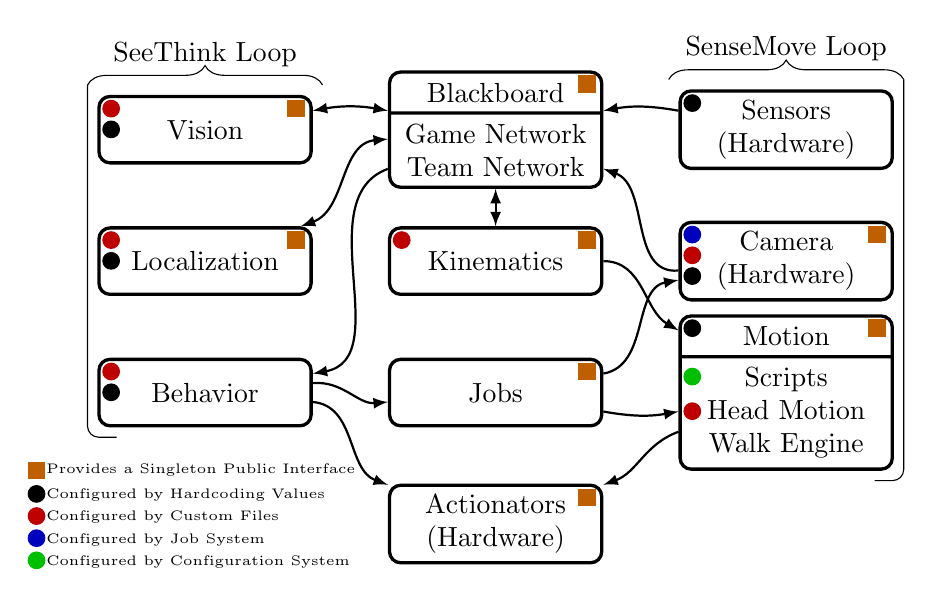
\begin{tikzpicture}[
			x=10.5em,y=4.75em,
			component/.style={
				rectangle
				, rounded corners
				, draw=black, very thick
				, text width=7em
				, minimum height=2.4em
				, text centered
			}
			, splitcomponent/.style={
				component
				, rectangle split
				, rectangle split parts=2
			}
			, configsystemconfig/.style={ color=green!75!black }
			, fileconfig/.style={ color=red!75!black }
			, jobconfig/.style={ color=blue!75!black }
			, hardcodedconfig/.style={ color=black }
			, publicinterface/.style={ color=orange!75!black}
			, write/.style={ ->, thick}
			, read/.style={<-, thick}
			, readwrite/.style={<->, thick}
			, >=latex
		]

		%\node at (0.5,2.5) {$P_{1}$};

		%%% Nodes
		%% Left hand Side
		\node at (0,3) [component] (vision) {Vision};
		\node at (0,2) [component] (localization) {Localization};
		\node at (0,1) [component] (behavior) {Behavior};

		%% Center
		\node at (1, 3) [splitcomponent] (blackboard) {Blackboard \nodepart{two} Game Network\\Team Network};
		\node at (1, 2) [component] (kinematics) {Kinematics};
		\node at (1, 1) [component] (jobs) {Jobs};
		\node at (1, 0) [component] (actionators) {Actionators (Hardware)};

		%% Right hand side
		\node at(2,3) [component] (sensors) {Sensors (Hardware)};
		\node at(2,2) [component] (camera) {Camera (Hardware)};
		\node at(2,1) [splitcomponent] (motion) {Motion \nodepart{two} Scripts\\Head Motion\\Walk Engine};

		%%% Connections
		%% Left side connections
		\path [readwrite, out=10, in=170] (vision) edge (blackboard);
		\path [readwrite, out=20, in=185] (localization) edge (blackboard);
		\path [read, out=10, in=200] (behavior) edge (blackboard);
		\path [write, out=5, in=185] (behavior) edge (jobs);
		\path [write, out=-5, in=160] (behavior) edge (actionators);
		
		%% Center connections
		\path [readwrite] (kinematics) edge (blackboard);

		%% Right side connections
		\path [write, out=170, in=10] (sensors) edge (blackboard);
		\path [write, out=185, in=-20] (camera) edge (blackboard);
		\path [write, out=-10, in=190] (jobs) edge (motion);
		\path [write, out=10, in=190] (jobs) edge (camera);
		\path [write, out=200, in=20] (motion) edge (actionators);
		\path [read, out=150, in=0] (motion) edge (kinematics);
		
		%%% Configuration Colours
		%% Vision
		\filldraw[fileconfig] ([yshift=-.5em,xshift=.5em]vision.north west) circle (3pt);
		\filldraw[hardcodedconfig] ([yshift=-1.25em,xshift=.5em]vision.north west) circle(3pt);
		\filldraw[publicinterface] ([yshift=-.8em,xshift=-0.9em]vision.north east) rectangle ++(6pt, 6pt);	
		
		%% Localization
		\filldraw[fileconfig] ([yshift=-.5em,xshift=.5em]localization.north west) circle(3pt);
		\filldraw[hardcodedconfig] ([yshift=-1.25em,xshift=.5em]localization.north west) circle (3pt);
		\filldraw[publicinterface] ([yshift=-.8em,xshift=-0.9em]localization.north east) rectangle ++(6pt, 6pt);
		
		%% Behavior
		\filldraw[fileconfig] ([yshift=-.5em,xshift=.5em]behavior.north west) circle(3pt);
		\filldraw[hardcodedconfig] ([yshift=-1.25em,xshift=.5em]behavior.north west) circle(3pt);
		
		%% Blackboard
		\filldraw[publicinterface] ([yshift=-.8em,xshift=-0.9em]blackboard.north east) rectangle ++(6pt, 6pt);
		
		%% Kinematics
		\filldraw[fileconfig] ([yshift=-.5em,xshift=.5em]kinematics.north west) circle(3pt);
		\filldraw[publicinterface] ([yshift=-.8em,xshift=-0.9em]kinematics.north east) rectangle ++(6pt, 6pt);
		
		%% Jobs
		\filldraw[publicinterface] ([yshift=-.8em,xshift=-0.9em]jobs.north east) rectangle ++(6pt, 6pt);
		
		%% Actionators
		\filldraw[publicinterface] ([yshift=-.8em,xshift=-0.9em]actionators.north east) rectangle ++(6pt, 6pt);
		
		%% Sensors
		\filldraw[hardcodedconfig] ([yshift=-.5em,xshift=.5em]sensors.north west) circle(3pt);
		
		%% Camera
		\filldraw[jobconfig] ([yshift=-.5em,xshift=.5em]camera.north west) circle(3pt);
		\filldraw[fileconfig] ([yshift=-1.25em,xshift=.5em]camera.north west) circle(3pt);
		\filldraw[hardcodedconfig] ([yshift=-2em,xshift=.5em]camera.north west) circle (3pt);
		\filldraw[publicinterface] ([yshift=-.8em,xshift=-0.9em]camera.north east) rectangle ++(6pt, 6pt);
		
		%% Motion
		\filldraw[hardcodedconfig] ([yshift=-.5em,xshift=.5em]motion.north west) circle (3pt);
		\filldraw[configsystemconfig] ([yshift=-2.25em,xshift=.5em]motion.north west) circle (3pt);
		\filldraw[fileconfig] ([yshift=-3.5em,xshift=.5em]motion.north west) circle(3pt);
		\filldraw[publicinterface] ([yshift=-.8em,xshift=-0.9em]motion.north east) rectangle ++(6pt, 6pt);
		
		%%% Legend
		\coordinate (legendpoint) at (.55, .35);
		
		%% Public Interface
		\node [below=3pt of legendpoint,anchor=south east] (publicinterfacelabel) {\tiny Provides a Singleton Public Interface};
		\filldraw[publicinterface] ([yshift=-3pt,xshift=-3pt]publicinterfacelabel.west) rectangle ++(6pt, 6pt);

		%% Hard Coded Config
		\node [below=0.9em of publicinterfacelabel.south west,anchor=south west] (hardcodedconfiglabel) {\tiny Configured by Hardcoding Values};
		\filldraw[hardcodedconfig] ([yshift=.5pt]hardcodedconfiglabel.west) circle (3pt);
		
		%% File Config
		\node [below=0.8em of hardcodedconfiglabel.south west,anchor=south west] (fileconfiglabel) {\tiny Configured by Custom Files};
		\filldraw[fileconfig] ([yshift=.5pt]fileconfiglabel.west) circle (3pt);

		%% Job Config
		\node [below=0.8em of fileconfiglabel.south west,anchor=south west] (jobconfiglabel) {\tiny Configured by Job System};
		\filldraw[jobconfig] ([yshift=.5pt]jobconfiglabel.west) circle (3pt);

		%% Config System Config
		\node [below=0.8em of jobconfiglabel.south west,anchor=south west] (configsystemconfiglabel) {\tiny Configured by Configuration System};
		\filldraw[configsystemconfig] ([yshift=.5pt]configsystemconfiglabel.west) circle (3pt);
		
		%%% Decorations
		%% SeeThink header
		\node[fit=(vision)(localization)(behavior)](leftgroup){};
		\draw[rounded corners] 
		(leftgroup.north west)--(leftgroup.south west) -- ++(0.10,0);			
		\draw[decorate,decoration={amplitude=7pt,brace}] % Header line
		(leftgroup.north west) -- (leftgroup.north east);

		\node[above=1.1em of leftgroup,anchor=center]{SeeThink Loop};

		%% SenseMove header
		\node[fit=(sensors)(camera)(motion)](rightgroup){};
		\draw[rounded corners] 
		(rightgroup.north east) -- (rightgroup.south east) -- ++(-0.10,0);
		\draw[decorate,decoration={amplitude=7pt,brace}]
		(rightgroup.north west) -- (rightgroup.north east);
		\node[above=1.1em of rightgroup,anchor=center]{SenseMove Loop};
	\end{tikzpicture}

\end{frame}

\begin{frame}
	\frametitle{Existing Architecture - Dependency Graph}
	\begin{adjustbox}{max totalsize={\textwidth}{.9\textheight},center}
	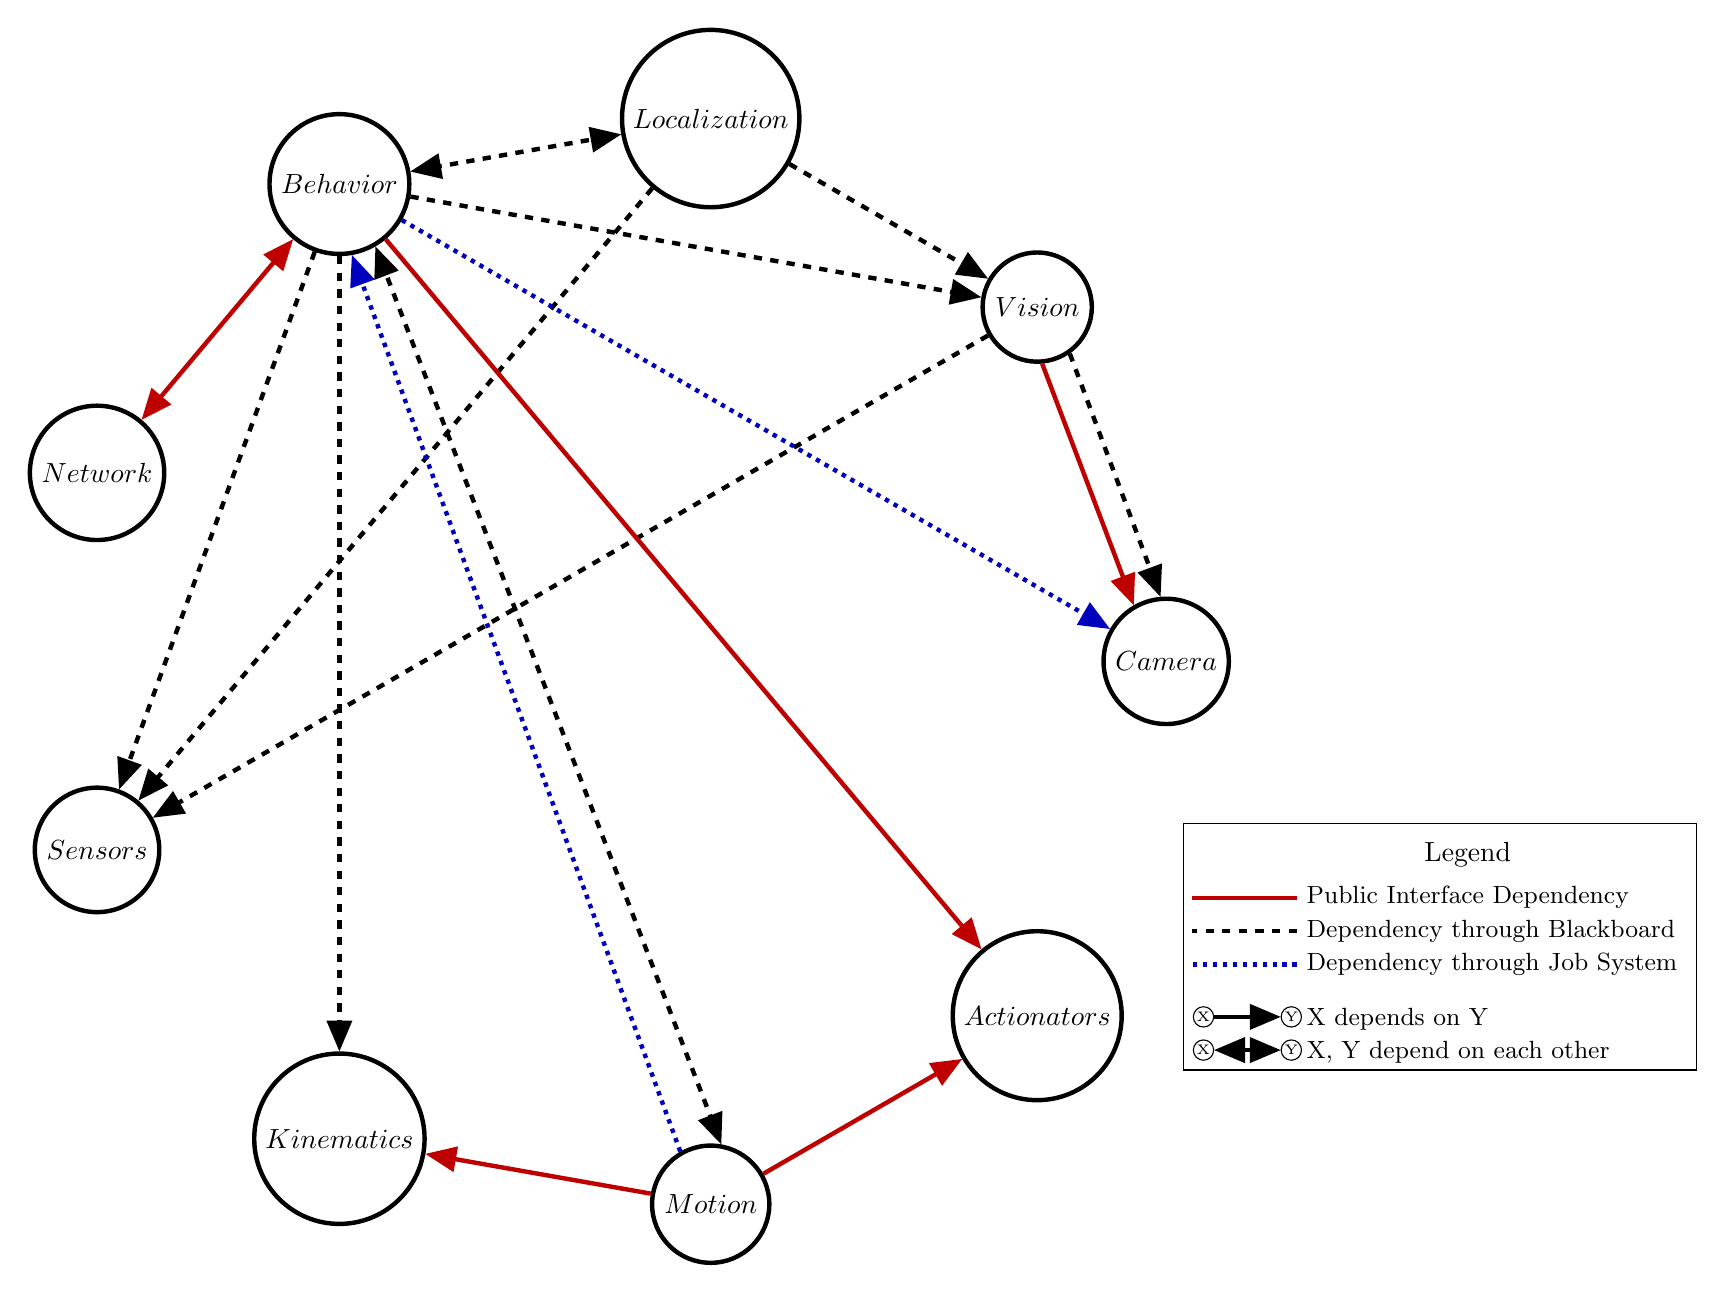
\begin{tikzpicture}[
		reactor/.style={draw, circle, ultra thick}
		, basearrow/.style={>=triangle 45, ultra thick}
		, blackboard/.style={basearrow, dashed}
		, publicinterface/.style={basearrow, color=red!75!black}
		, jobs/.style={basearrow, dotted, color=blue!75!black}
		, dependent/.style={->}
		, codependent/.style={<->}]

		%%% Legend
		\coordinate (legendpoint) at (13, -2);

		%% Public Interface Dependency
		\node [below=of legendpoint,anchor=east] (publicinterfacelabel) {\small Public Interface Dependency};
		\draw [publicinterface] (publicinterfacelabel.mid west) -- ++(-38pt, 0pt);

		%% Blackboard Dependency
		\node [below=12pt of publicinterfacelabel.south west,anchor=south west] (blackboardlabel) {\small Dependency through Blackboard};
		\draw[blackboard] (blackboardlabel.mid west) -- ++(-38pt, 0pt);

		%% Jobs Dependency
		\node [below=12pt of blackboardlabel.south west,anchor=south west] (joblabel) {\small Dependency through Job System};
		\draw[jobs] (joblabel.mid west) -- ++(-38pt, 0pt);

		%% Dependancy Type: Depends on
		\node[below=20pt of joblabel.south west,anchor=south west] (dependencylabel) {\small X depends on Y};
		\node[circle, draw, inner sep=0.5pt] (dependencynodeY) at ([yshift=1pt,xshift=-2pt]dependencylabel.mid west) {\tiny Y};
		\node[circle, draw, inner sep=0.5pt, left=24pt of dependencynodeY] (dependencynodeX) {\tiny X};
		\draw[basearrow, dependent] (dependencynodeX) edge (dependencynodeY);

		%% Dependancy Type: Codependent
		\node[below=12pt of dependencylabel.south west,anchor=south west] (codependencylabel) {\small X, Y depend on each other};
		\node[circle, draw, inner sep=0.5pt] (codependencynodeY) at ([yshift=1pt,xshift=-2pt]codependencylabel.mid west) {\tiny Y};
		\node[circle, draw, inner sep=0.5pt, left=24pt of codependencynodeY] (codependencynodeX) {\tiny X};
		\draw[basearrow, codependent] (codependencynodeX) edge (codependencynodeY);

		%% Legend Header
		\node[above=0pt of publicinterfacelabel] (legendheader) {Legend};

		%%% Draw all of our components in a circle
		\foreach [count=\i] \reactor in {Camera, Vision, Localization, Behavior, Network, Sensors, Kinematics, Motion, Actionators} {
		
			% Draw the reactors around the central star
			\node[reactor] (\reactor) at ({360/9 * (\i - 1)}:7cm) {$\reactor$};
		};

		%% Legend Border
		\node[fit=(legendheader)(publicinterfacelabel)(blackboardlabel)
				(joblabel)(dependencylabel)(codependencynodeX)(codependencynodeY),rectangle,draw](legendgroup){};

		%%% Dependencies
		%% Vision
		\path[blackboard, dependent] (Vision.305) edge (Camera.95);
		\path[publicinterface, dependent] (Vision.275) edge (Camera.120);
		\path[blackboard, dependent] (Vision) edge (Sensors);

		%% Localization
		\path[blackboard, dependent] (Localization) edge (Sensors);
		\path[blackboard, dependent] (Localization) edge (Vision);

		%% Behavior
		\path[blackboard, codependent] (Behavior) edge (Localization);
		\path[blackboard, dependent] (Behavior) edge (Kinematics);
		\path[blackboard, dependent] (Behavior) edge (Vision);
		\path[blackboard, dependent] (Behavior) edge (Sensors);
		\path[publicinterface, dependent] (Behavior) edge (Actionators);
		\path[publicinterface, codependent] (Behavior) edge (Network);
		\path[jobs, dependent] (Behavior) edge (Camera);

		%% Motion
		\path[blackboard, codependent] (Motion.80) edge (Behavior.300);
		\path[jobs, dependent] (Motion.120) edge (Behavior.280);
		\path[publicinterface, dependent] (Motion) edge  (Actionators);
		\path[publicinterface, dependent] (Motion) edge (Kinematics);
	\end{tikzpicture}
	\end{adjustbox}
\end{frame}

\subsection{Justification for Change}
\begin{frame}
	\frametitle{Problems in Existing System}
	\begin{itemize}
		\item Hidden Dependencies
			\begin{itemize}
				\item The existing systems dependencies are very poorly defined
				\item For example, localizations dependency on the Stationary/Mobile object system.
				\item These hidden dependencies make it difficult to work on a system without understanding the whole system
			\end{itemize}
	
		\item Threading Issues
			\begin{itemize}
				\item Current system does not handle synchronisation between the two threads well
				\item e.g. The kick system can be prompted mid way by the walk engine, the two can even run together resulting in the robot standing still for prolonged periods.
				\item Happens because the interactions between the two threads is undefined in most cases
			\end{itemize}
	\end{itemize}
\end{frame}

\begin{frame}
	\frametitle{Problems in Existing System}
	\begin{itemize}			
		\item Network Communication
			\begin{itemize}
				\item Network communication is currently entirely through Localisation and Behaviour
				\item Adding new network communication requires modifying these two systems
				\item Because of the difficulty of adding new networking, no new networking will be added
			\end{itemize}
			
		\item Build System
			\begin{itemize}
				\item The current build system uses a make file that calls cmake that builds a make file that is called by the original make file
				\item This makes adding and removing components to the system in a meaningful way difficult
			\end{itemize}
	\end{itemize}
\end{frame}

\begin{frame}
	\frametitle{Useful Features}
	\begin{itemize}
		\item Modular Design
			\begin{itemize}
				\item Many modules that are made for robotics (walk engine, script engine) are useful for more then just soccer.
				\item Being able to use Mock inputs allows the system to be tested without access to a robot
				\item Being able to compose various modules into a binary would allow the robot to do more
				\item Enabling the sharing of these modules between researchers would result in better development (more people using the same code)
			\end{itemize}
			
		\item Transparent Multithreading
			\begin{itemize}
				\item Modern CPUs are getting more cores, rather then becoming faster
				\item Threading is difficult and can almost never be sensibly done at the module level
				\item Threading should be handled by the architecture in a way that can scale up to many cores
			\end{itemize}
	\end{itemize}
\end{frame}
			
\begin{frame}
	\frametitle{Useful Features}
	\begin{itemize}
		\item Runtime Statistics
			\begin{itemize}
				\item When optimising programs for speed it is useful to see how long each section of the code took
				\item Breaking up the modules and timing their execution better shows where CPU time is being used
			\end{itemize}
			
		\item Fine Grained Debugging
			\begin{itemize}
				\item When debugging a large system, there is often a low signal to noise ratio as a lot of debug lines are not useful
				\item Splitting up log lines based on source can help identify problems
				\item Being able to view the call graph in real time on a repeated process helps to identify links
			\end{itemize}
	\end{itemize}
\end{frame}

%----------------------------------------------------------------------------------------
\section{C++ Review}
%----------------------------------------------------------------------------------------
\subsection{Smart Pointers and Move Semantics}
\begin{frame}
	\frametitle{C++ Review: Smart Pointers}
	\begin{itemize}
		\item Smart Pointers automatically handle releasing pointer memory for you.
		\item Different smart pointers decide who deletes data and when it gets deleted.
		\item As of C++11 there is almost never a reason to use new/delete or raw pointers.
		\item Instead you should use std::unique\_ptr and std::shared\_ptr with std::make\_shared and std::make\_unique
		\item In NUClear you will primarily use std::unique\_ptr to send messages.
	\end{itemize}
\end{frame}

\begin{frame}
	\frametitle{C++ Review: std::unique\_ptr}
	\begin{itemize}
		\item Only one unique\_ptr is allowed to point to a particular address.
		\item When copied the unique\_ptr transfers ownership to the new unique\_ptr and the old one becomes invalid.
		\item When you pass a unique\_ptr to a function you are giving away it's ownership.
		\item Don't use a unique\_ptr after it has been passed or copied. It will be null!
		\item unique\_ptr deletes it's data when it goes out of scope. 
		\item This should be your go-to pointer unless you have a good reason otherwise.
	\end{itemize}
\end{frame}

\begin{frame}
	\frametitle{C++ Review: std::move}
	\begin{itemize}
		\item Data stealing in C++ is known as "move semantics"
		\item It's a fancy way of expressing transfer of ownership.
		\item When something is "moved" it can't be used after moving.
		\item Compilers automatically move things that don't have a name.
		\item Some classes can only be constructed by moving data into them. Like std::unique\_ptr!
		\item When something has a name you use std::move(...) to move it!
	\end{itemize}
\end{frame}

\begin{frame}[fragile]
	\frametitle{C++ Review: std::move}
	\begin{lstlisting}[language=nuclear]
		// We don't use raw pointers but this is a slide!
		int* chump = new data(5);

		// Prints 5.
		std::cout << *chump << std::endl;

		// theif steals 5 from chump.
		int* thief = std::move(chump);

		// Error: Chump doesn't have 5 anymore.
		std::cout << *chump << std::endl;

		// No problem: Thief stole 5.
		std::cout << *thief << std::endl;
	\end{lstlisting}
\end{frame}

\begin{frame}[fragile]
	\frametitle{C++ Review: std::unique\_ptr}

	std::unique\_ptr uses move semantics!	

	\begin{lstlisting}[language=nuclear]
		#include <memory> // unique_ptr & shared_ptr

		void processImage(const Image& image) {
		    std::unique_ptr<MyData> chump = 
		        std::make_unique<MyData>();

		    chump->something; // Access pointer-style:* and ->
			
		    // theif has stolen chump's pointer.
		    // you can't use chump to get to the
		    // data since he doesn't have it.
		    std::unique_ptr<MyData> thief = std::move(data); 
		    thief->something; // No problem!
		    chump->something; // Error. Bad chump!
		} // thief automatically releases memory here. 
	\end{lstlisting}
\end{frame}

\begin{frame}[fragile]
	\frametitle{C++ Review: std::shared\_ptr}
	\begin{itemize}
		\item shared\_ptr is a reference counting pointer.
		\item When no shared\_ptr's point to a particular bit of data it will be deleted.
		\item When you copy a shared\_ptr it increments a shared reference counter. 
		\item When a shared\_ptr falls out of scope is decrements the shared reference counter.
		\item When the counter is zero your data is deleted.
		\item shared\_ptr should be used when you truly need to share data and there is no clear single-owner. 
			This is more rare then people might like to believe.
	\end{itemize}
\end{frame}

\subsection{Templates}
\begin{frame}
	\frametitle{C++ Review: Templates}
	\begin{itemize}
		\item Templates let you write type-agnostic code.
		\item Briefly touched on in SENG1120.
		\item Templates let you provide a "blueprint" for a function or class allowing the compiler to generate
			copies of the same class that vary based on what type they are templated with.
		\item For example the std::vector class is a template which lets the compiler generate a concrete
			std::vector$<$int$>$ or std::vector$<$MyClass$>$ on demand when a user tries to use those classes 
			in a vector.
	\end{itemize}
\end{frame}

\begin{frame}[fragile]
	\frametitle{C++ Review: Templates}
	\begin{lstlisting}[language=nuclear]
		// Works on anything that has an operator+
		template <typename T>
		T add(const T& first, const T& second) {
		    return first + second;
		}
		
		// Generates a "int" version of add at compile time.
		std::cout << add<int>(1, 2) << std::endl;

		// C++ can also automatically work out the T.
		std::cout << add(1.0, 5.0) << std::endl;

		// Behind the scenes C++ generates something like this
		// for add<int>
		int add(const int& first, const int& second) {
		    return first + second;
		}
	\end{lstlisting}
\end{frame}

\subsection{Template Metaprogramming}
\begin{frame}
	\frametitle{C++ Review: Template Metaprogramming}
	\begin{itemize}
		\item Clever people realized that templates are actually turing complete.
		\item You can write some really interesting programs with templates and perform logic at compile time.
		\item Since this was an accident the syntax isn't super-friendly.
		\item However you can use Template Metaprogramming to express complex problems with no runtime cost.
		\item We use this extensively in NUClear but avoid it in the robocup code.
		\item Except for configuration (looking at you Trent!).
	\end{itemize}
\end{frame}

\begin{frame}[fragile]
	\frametitle{C++ Review: Calling template functions}
	\begin{itemize}
		\item NUClear's On and Emit functions look weird to new C++ programmers as they contain a lot of arguments in angle brackets 
			$<>$ instead of the expected round braces ().
		\item The easiest way to think about this is angle bracket arguments are evaluated at compile time while round braces are
			evalutaed at runtime. 
	\end{itemize}

	\begin{lstlisting}[language=nuclear]
		//	      <Compile>(Runtime)
		something<1, 2, 3>(4, 5, 6);

		// 1, 2 and 3 will be evaluated when the program 
		// is compiled and as such can't change based on
		// user input. 4, 5 and 6 are regular parameters.
	\end{lstlisting}
\end{frame}

%----------------------------------------------------------------------------------------
\section{NUClear Architecture}
%----------------------------------------------------------------------------------------
\subsection{Architectural Overview}
\begin{frame}
	\frametitle{Message Passing}
	\begin{itemize}
		\item NUClear is a message passing system
		\item Rather then directly interacting with each-other, indirectly interact through common data
		\item Results in very loose coupling making it easy to add remove or change components
		\item Makes it easy to have multiple components using the same input data
	\end{itemize}
\end{frame}

\begin{frame}
	\frametitle{Multi Threading}
	\begin{itemize}
		\item NUClear is a multi threaded framework
		\item It will transparently multithread any code that is given to it
		\item This allows it to make use of all of the resources in the system
		\item Synchronisation needs to be taken into account if multiple threads could access the same data
	\end{itemize}
\end{frame}

\begin{frame}
	\frametitle{Powerplant}
	\begin{itemize}
		\item The Powerplant is the core component of the NUClear system
		\item It is the central datapoint for the whole system
		\item It holds the functionality for doing the following:
			\begin{itemize}
				\item Install a new reactor
				\item Start up the system
				\item Shutdown the system
			\end{itemize}
		\item You are also able to directly send messages from it (for injecting messages)
		\item Most of the time, you will never directly interact with it
	\end{itemize}
\end{frame}

\begin{frame}
	\frametitle{Reactor}
	\begin{itemize}
		\item A Reactor is the primary method that you will interact with the system
		\item It is a class that extends from NUClear::Reactor
		\item It has all of the methods on it that are used to listen for and emit messages, these being:
			\begin{itemize}
				\item on
				\item emit
				\item log
			\end{itemize}
		\item You then install these reactors into the Powerplant
	\end{itemize}
\end{frame}

\begin{frame}
	\frametitle{Reaction}
	\begin{itemize}
		\item A reaction is a single function that is run in response to new data
		\item They take as arguments constant references to the data that they use
		\item The data that is passed into a reaction function can be considered thread safe
		\item The lifetime of the data used is managed by the Powerplant 
			\begin{itemize}
				\item If you really need to save the data, you will need to save a copy
			\end{itemize}
	\end{itemize}
\end{frame}

\begin{frame}
	\frametitle{Smart Types}
	\begin{itemize}
		\item Smart Types are special types that when used in an on statement will cause different behaviour
		\item Built into NUClear there are the smart types Every, Last, and Network
		\item The Configuration System also provides the Configuration smart type
	\end{itemize}
\end{frame}

\begin{frame}
	\frametitle{Extension}
	\begin{itemize}
		\item The creation of new Smart Types is done through extension
		\item Extension allows you to change the way specific datatypes are handled when:
			\begin{itemize}
				\item Exists: The data type is used in an on statement
				\item Emit: Data is emitted (particular data types and whole scopes)
				\item TriggerType: What datatype will cause a reaction to run
				\item Get: Data is retrieved (can even return a different datatype)
			\end{itemize}
		\item Extensions are generally for when system wide common functionality is needed
		\item They are advanced usage and should not be the normal usage pattern
	\end{itemize}
\end{frame}

\begin{frame}
	\frametitle{Service Thread}
	\begin{itemize}
		\item Sometimes a whole thread is needed to listen to an external blocking source
			\begin{itemize}
				\item An example would be a user interface
			\end{itemize}
		\item However having NUClear manage the lifetime of the program is beneficial
		\item To allow this you can create service threads
		\item These threads have a run() and kill() method which start and stop the thread respectively
		\item Most use cases should not need these and should be triggered by events if possible
	\end{itemize}
\end{frame}

\begin{frame}[fragile]
	\frametitle{NUClear Architecure}
	\begin{adjustbox}{max totalsize={\textwidth}{.9\textheight},center}
	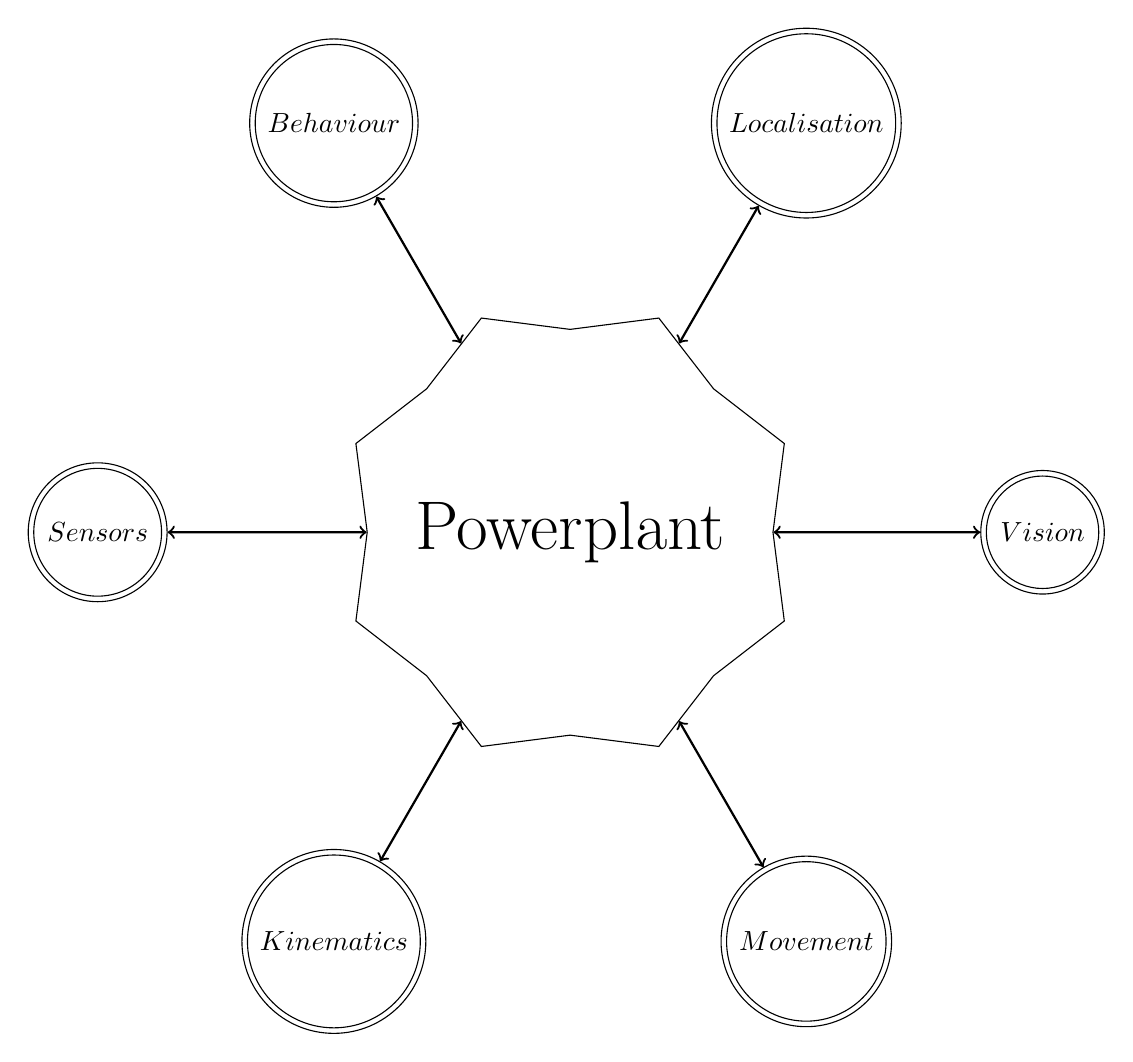
\begin{tikzpicture}[
		old inner xsep/.estore in=\oldinnerxsep,
		old inner ysep/.estore in=\oldinnerysep,
		double circle/.style 2 args={
			circle,
			old inner xsep=\pgfkeysvalueof{/pgf/inner xsep},
			old inner ysep=\pgfkeysvalueof{/pgf/inner ysep},
			/pgf/inner xsep=\oldinnerxsep+#1,
			/pgf/inner ysep=\oldinnerysep+#1,
			alias=sourcenode,
			append after command={
			let \p1 = (sourcenode.center),
				\p2 = (sourcenode.east),
				\n1 = {\x2-\x1-#1-0.5*\pgflinewidth}
			in
				node [inner sep=0pt, draw, circle, minimum width=2*\n1,at=(\p1),#2] {}
			}
		}
		, double circle/.default={2pt}{black}
		, reactor/.style={draw, double circle}
		, readwrite/.style={<->, thick}
	]
	
	% Draw our central Power Plant star
	\node [draw,star,star points=8,star point ratio=0.875,minimum width=5cm] (powerplant) {\Huge Powerplant};
	
	% Loop through each of our reactors
	\foreach [count=\i] \reactor in {Vision,Localisation,Behaviour,Sensors,Kinematics,Movement} {
	
		% Draw the reactors around the central star
		\node[draw,reactor] (reactorcircle) at ({360/6 * (\i - 1)}:6cm) {$\reactor$};
	
		% Draw a line from our reactor to our powerplant
		\path[readwrite] (reactorcircle) edge (powerplant);
	};
	\end{tikzpicture}
	\end{adjustbox}

\end{frame}

\subsection{Key Functions}
\begin{frame}[fragile]
	\frametitle {Key Functions: On and Trigger}
	\begin{itemize}
		\item Q: "I want to do something when new data is available"
		\item A: Use On and Trigger!
		\item Notifies Power Plant that you are interested in specific data and triggers a callback when new data is available.
	\end{itemize}

	\begin{lstlisting}[language=nuclear]
		// Make sure to take arguments by const reference!
		void processImage(const Image& data) {
		    // Do something with the image data here.
		}

		// Tells PowerPlant to call processImage when new
		// image data is available.
		on<Trigger<Image>>(processImage);
	\end{lstlisting}
\end{frame}

\begin{frame}[fragile]
	\frametitle {Key Functions: With}
	\begin{itemize}
		\item Q: "I want to access data other then the one I triggered on"
		\item A: Use With!
		\item Notifies Power Plant that you want the latest version of some other data when your trigger function is called.
	\end{itemize}

	\begin{lstlisting}[language=nuclear]
		// Order of arguments needs to match the order of 
		// Trigger and With arguments.
		void processData(
		    const Image& image,
		    const SensorData& sensors) {
		    // Do something with image and sensors
		}

		// Calls process data when a new image frame is 
		// captured. Also passes the most recent sensordata
		// to processData.
		on<Trigger<Image>, With<SensorData>>(processData);
	\end{lstlisting}
\end{frame}

\begin{frame}[fragile]
	\frametitle {Key Functions: With}
	\begin{itemize}
		\item Q: "I need more then one data!"
		\item A: With can take multiple arguments!
	\end{itemize}

	\begin{lstlisting}[language=nuclear]
		void processData(
		    const Image& image,
		    const SensorData& sensors,
		    const AudioData& audio) {
		    // Do stuff with image, sensors and audio.
		}

		// We can either use With multiple times or With<A,B>
		on<Trigger<Image>, 
		   With<SensorData, AudioData>>(processData);
		on<Trigger<Image>, 
		   With<SensorData>, With<AudioData>>(processData);
	\end{lstlisting}
\end{frame}

\begin{frame}
	\frametitle {Key Functions: Options}
\end{frame}

\begin{frame}
	Options
\end{frame}

\begin{frame}
	\frametitle{Key Functions Emit}
	Default
	Scopes
	Unique Pointers
	Code Example
\end{frame}

\begin{frame}
	\frametitle{Key Functions Log}
	Stream operator overload
	variardic
\end{frame}

\begin{frame}[fragile]
	\frametitle{Complete Reactor Example}
		
	\begin{lstlisting}[language=nuclear]
	// Vision.h
	class Vision : public NUClear::Reactor {
	public:
	    Vision(NUClear::PowerPlant* plant);
	};
	\end{lstlisting}
	
	\begin{lstlisting}[language=nuclear]
	// Vision.cpp
	Vision::Vision(NUClear::PowerPlant* plant)
	: Reactor(plant) {        
	    on<Trigger<Image>>
	    ([this](const Image& image) {
	        // Make a classified image and emit it
	        auto classified = std::make_unique<ClassifiedImage>(makeClassified(image));
	        emit(std::move(classified));
	    });
	}
	\end{lstlisting}
\end{frame}

\subsection{Smart Types}
\begin{frame}[fragile]
	\frametitle{Smart Types - Every}
	\begin{itemize}
		\item The every smart type is used to have an event triggered at a regular interval
		\item The first argument is the number of time units to wait
		\item The second argument is the time unit that we are using
		\begin{itemize}
			\item This is a member of std::chrono::duration (milliseconds, microseconds etc...)
		\end{itemize}
	\end{itemize}

	\begin{lstlisting}[language=nuclear]
	using std::chrono::milliseconds;
	on<Trigger<Every<100, milliseconds>>>(
	[](const time_t& t) {
	    // Do something every 100 milliseconds!
	});
	\end{lstlisting}
\end{frame}

\begin{frame}[fragile]
	\frametitle{Smart Types - Last}
	\begin{itemize}
		\item The last smart type will get you the last N emitted values of a type
		\item The first argument is the number of elements to get (at most)
		\item The second argument is the type of data to get
		\item It will give you as many as the system has (up to a max)
		\item The type of data that you get back is a vector of pointers (the LastList$<$type$>$ is there for convenience)
	\end{itemize}
	
	\begin{lstlisting}[language=nuclear]
	on<Trigger<Last<5, Image>>>(
	[](const LastList<Image>& list) {
	    // LastList is a vector of pointers to the last 5 Images
	});
	\end{lstlisting}
\end{frame}

\begin{frame}[fragile]
	\frametitle{Smart Types - Network}
	\begin{itemize}
		\item The Network smart type will get you network events of a particular type
		\item The data will come from all of the other systems on your network
		\item Each Network object contains both the data, and the source of the data
	\end{itemize}
	
	\begin{lstlisting}[language=nuclear]
	on<Trigger<Network<BallLocation>>>(
	[](const Network<BallLocation>& ball) {
	    // We get all the ball locations emitted to the network
	});
	\end{lstlisting}
\end{frame}

\begin{frame}[fragile]
	\frametitle{Smart Types - Configuration}
	\begin{itemize}
		\item Configuration is a smart type that will read Configuration files from the config directory
		\item Configurations will trigger every time the file is modified
		\item They contain a datatype called config which can be automagically typed to any data it knows about
	\end{itemize}
	
	\begin{lstlisting}[language=nuclear]
	struct MyConfigPath {
	    static constexpr char* path = "Mine.json";
	}
	
	on<Trigger<Configuration<MyConfigPath>>>(
	[](const Configuration<MyConfigPath>& config) {
	    // config.name has the name of the file
	    // config.config has our configuration
	});
	\end{lstlisting}
\end{frame}

\begin{frame}[fragile]
	\frametitle{Smart Types - Configuration}
	
	\begin{itemize}
		\item Configurations can also be set as directories
		\item In this case they will emit an event for every item in the directory
		\item They will emit events whenever an element is added or modified in that directory
	\end{itemize}
	
	\begin{lstlisting}[language=nuclear]
	struct Scripts {
	    static constexpr char* path = "scripts/";
	}
	
	on<Trigger<Configuration<Scripts>>>(
	[](const Configuration<MyConfigPath>& config) {
	    // config.name has the name of the script
	    // config.config has the script configuration
	});
	\end{lstlisting}
\end{frame}

%----------------------------------------------------------------------------------------
\section{NUClear Powered Robocup}
%----------------------------------------------------------------------------------------
\begin{frame}
	\frametitle{Project Directory Structure}
	Project Directory Structure
\end{frame}

\subsection{Antipatterns}
\begin{frame}[fragile]
	\frametitle{Infinite Looping Reaction}

	\begin{itemize}
		\item Never do an infinite loop in a reaction
		\item It ties up a thread pool thread and can eventually kill the system
		\item You should always be able to trigger on either an every or another event
		\item In the rare case that you do need to loop forever, use a service thread
	\end{itemize}

	\begin{lstlisting}[language=nuclear]
	on<Trigger<MyData>>([](const MyData& data) {
	    // Bad! You've killed a thread pool thread!
	    while(true) {
	        doSomething(data);
	    }
	}
	\end{lstlisting}
\end{frame}

\begin{frame}[fragile]
	\frametitle{Data Hog}

	\begin{itemize}
		\item Whenever it makes sense, emit data rather then using it
		\item For example, if vision makes a classified image, this could be useful
		\item Rather then immediately using this classified image, we can emit and trigger on it
		\item This way others can use this data as well as us
	\end{itemize}

	\begin{lstlisting}[language=nuclear]
	on<Trigger<Image>>([](const Image& image) {
	
	    // This could be emitted for others to use
	    // Saving them the trouble of recoding or copying code
	    auto classified = makeClassifiedImage(image);
		
	    auto seenObjects = findObjects(classified)
	}
	\end{lstlisting}
\end{frame}

\subsection{Module Examples}
\begin{frame}
	\frametitle{Some title}
	Config System
	Party Darwin
	Show examples
\end{frame}

\subsection{Current Porting Status}
\begin{frame}
	\frametitle{Current Porting Status}
	What has been ported
\end{frame}

\end{document} 
